%% ----------------------------------------------------------------
%% Thesis.tex -- MAIN FILE (the one that you compile with LaTeX)
%% ---------------------------------------------------------------- 

% Set up the document
\documentclass[a4paper, 11pt, oneside]{Thesis}  % Use the "Thesis" style, based on the ECS Thesis style by Steve Gunn
\graphicspath{Figures/}  % Location of the graphics files (set up for graphics to be in PDF format)

% Include any extra LaTeX packages required
\usepackage[square, numbers, comma, sort&compress]{natbib}  % Use the "Natbib" style for the references in the Bibliography
\usepackage{verbatim}  % Needed for the "comment" environment to make LaTeX comments
\hypersetup{urlcolor=blue, colorlinks=true}  % Colours hyperlinks in blue, but this can be distracting if there are many links.

%% ----------------------------------------------------------------
\begin{document}
\frontmatter      % Begin Roman style (i, ii, iii, iv...) page numbering

% Set up the Title Page
\title  {Title}

\authors {Gubler Fabian}
\addresses  {\groupname\\\deptname\\\univname}  % Do not change this here, instead these must be set in the "Thesis.cls" file, please look through it instead

\maketitle
%% ----------------------------------------------------------------

\setstretch{1.3}  % It is better to have smaller font and larger line spacing than the other way round

% Define the page headers using the FancyHdr package and set up for one-sided printing
\fancyhead{}  % Clears all page headers and footers
\rhead{\thepage}  % Sets the right side header to show the page number
\lhead{}  % Clears the left side page header

\pagestyle{fancy}  % Finally, use the "fancy" page style to implement the FancyHdr headers

%% ----------------------------------------------------------------
% The "Funny Quote Page"
\pagestyle{empty}  % No headers or footers for the following pages

\null\vfill
% Now comes the "Quote(s)", written in italics
\textit{“Cyber Currencies and the blockchain have the potential to radically transform the way we think about and interact with money, and to fundamentally change the structure of our economic and social systems.”}

\begin{flushright}
Vitalik Buterin (Founder of Ethereum)
\end{flushright}

\null\vfill
\textit{Encryption will have very serious consequences for law enforcement and national security agencies at all levels. Sophisticated criminals will come to count on these means of evading detection. It’s the equivalent of a closet that can’t be opened. A safe that can’t be cracked. And my question is, at what cost?}

\begin{flushright}
James Comey (Former Director of the FBI)
\end{flushright}



\vfill\vfill\vfill\vfill\vfill\vfill\null
\clearpage  % Quote page ended, start a new page
%% ----------------------------------------------------------------

% The Abstract Page
\addtotoc{Abstract}  % Add the "Abstract" page entry to the Contents
\abstract{
\addtocontents{toc}{\vspace{1em}}  % Add a gap in the Contents, for aesthetics

Lorem Ipsum


}

\clearpage  % Abstract ended, start a new page
%% ----------------------------------------------------------------

\setstretch{1.3}  % Reset the line-spacing to 1.3 for body text (if it has changed)

\pagestyle{fancy}  %The page style headers have been "empty" all this time, now use the "fancy" headers as defined before to bring them back


%% ----------------------------------------------------------------
\lhead{\emph{Contents}}  % Set the left side page header to "Contents"
\tableofcontents  % Write out the Table of Contents



%% ----------------------------------------------------------------
\setstretch{1.5}  % Set the line spacing to 1.5, this makes the following tables easier to read
\clearpage  % Start a new page

%% ----------------------------------------------------------------
% End of the pre-able, contents and lists of things

\addtocontents{toc}{\vspace{2em}}  % Add a gap in the Contents, for aesthetics


%% ----------------------------------------------------------------
\mainmatter	  % Begin normal, numeric (1,2,3...) page numbering
\pagestyle{fancy}  % Return the page headers back to the "fancy" style

% Include the chapters of the thesis, as separate files
\chapter{Introduction}
\lhead{\emph{Introduction}}  % Set the left side page header

% Cyber currencies, also known as cryptocurrencies, have gained significant attention in recent years due to their unique features and potential impact on the economy. These digital assets use cryptography for secure financial transactions and are facilitated through the use of a decentralized ledger, known as a blockchain. The anonymity and decentralized nature of cyber currencies have made them attractive to cybercriminals as a means of payment and exchange, leading to their use in a range of illicit activities such as money laundering, human trafficking, and drug trafficking (Böhme et al., 2015).

%%%%%%%%%%%%%%%%%%%%%%%%%%%%%%%%%
% Hook
%%%%%%%%%%%%%%%%%%%%%%%%%%%%%%%%%
Cyber currencies have attracted considerable attention in recent years due to their distinctive characteristics and potential economic impact. These virtual assets use cryptography to enable secure financial transactions and are facilitated through the use of a decentralized ledger, known as the blockchain. The anonymous and decentralized nature of cyber currencies has made them attractive for cybercriminals as a means of payment and exchange. In this regard, cyber currencies are facilitating a variety of illegal operations, such as money laundering, ransomware attacks, and drug trafficking \cite{bohme_bitcoin_2015} (p. 230).

%%%%%%%%%%%%%%%%%%%%%%%%%%%%%%%%%
% Relation to National Security
%%%%%%%%%%%%%%%%%%%%%%%%%%%%%%%%%
As stated in Satoshi Nakamoto's infamous white paper on bitcoin, one of the primary motivations for developing cyber currencies was to exist independently of a central authority or government \cite{nakamoto_bitcoin_nodate} (p. 4). Regardless of this intentional design decision, Bitcoin and similar currencies should not be viewed as separate from nation-states. Without a doubt, quite the contrary has been observed with regard to recent pressures to counteract its harmful influences in underground black markets and cybercrime \cite{ablon_markets_2014} (p. 4-6).

%%%%%%%%%%%%%%%%%%%%%%%%%%%%%%%%%
% State-driven Cyber Crime
%%%%%%%%%%%%%%%%%%%%%%%%%%%%%%%%%
Moreover, cyber currencies are increasingly being used to fund and support cybercrime, ranging from hacking and malware attacks to more sophisticated forms like economic espionage and sabotage \cite{reuter_information_2019} (p. 22). In particular, cyber currencies have been used as a tool in these kinds of crimes, because they provide the ability to create anonymous and untraceable transactions. 

%%%%%%%%%%%%%%%%%%%%%%%%%%%%%%%%%
\section{Research Questions}
%%%%%%%%%%%%%%%%%%%%%%%%%%%%%%%%%
The use of cyber currencies in cybercrime raises a number of critical issues and challenges that affect societies on a national and global scale. This thesis aims to address these questions through a review of relevant literature and analysis of case studies. The specific research questions for this study are: 
% TODO: Compare with Lecture Hints
\begin{enumerate}
    \item What types of cyber currencies are being used in cybercrime, and for what purposes?
    \item How are state actors involved in cybercrime, and what measures are being taken to combat them?
    \item How do state-driven actions influence the development of cyber currencies, and what are the future implications?
\end{enumerate}

%%%%%%%%%%%%%%%%%%%%%%%%%%%%%%%%%
\section{Structure of the Thesis}
%%%%%%%%%%%%%%%%%%%%%%%%%%%%%%%%%
To address these questions, the remaining chapters of this thesis are organized as follows:
% VERSION 2:2
The following chapter gives a definition of cyber currencies and a brief history of them, including the key features and traits that are unique to them. This will provide a foundational understanding for the rest of the thesis.
% VERSION 2:3 (Optional - Could merge with Ch. 2)
% In Chapter 2.2, the different types of cyber currencies used in state-sponsored cybercrime are explained, along with examples and their respective distinctions.
% VERSION 1:3
In Chapter 3, we examine how cyber currencies are used in cybercrime, including the use of specific cyber currencies.
% VERSION 1:4
Subsequently, Chapter 4 examines the measures taken by state actors to combat the use of cyber currencies in cybercrime, by looking at the challenges and examining regulatory frameworks as a potential solution.
Following, Chapter 4 investigates the measures taken by state actors to combat the use of cyber currencies in cybercrime by examining cyber currency specific challenges and discussing regulatory frameworks as a potential solution.
% VERSION 2:6
Further, Chapter 5 assesses the impact of cybercrime on the development of cyber currencies, by looking at according consequences for trust and innovation and the potential for increased regulation. 
% VERSION 2:7
Finally, Chapter 6 concludes with a summary of the study's key findings, as well as implications and suggestions for future research.


 
% \chapter{Background} \label{Chapter2}
\lhead{\emph{Background}}  % Set the left side page header


%%%%%%%%%%%%%%%%%%%%%%%%%%%%%%%%%
% Definition
%%%%%%%%%%%%%%%%%%%%%%%%%%%%%%%%%
Cyber currencies, also known as cryptocurrencies, are a peer-to-peer version of electronic cash that use cryptography to secure financial transactions \cite{nakamoto_bitcoin_nodate} (p. 1). They are decentralized, as they can be sent directly from one party to another without going through a financial institution, such as a bank or government. Instead, they rely on a distributed ledger technology known as a blockchain that enables transactions to be recorded and verified by a network of computers. \cite{universiti_utara_malaysia_robust_2018} (p. 24). In turn, this enables a secure and transparent transfer of value without the need for a centralized financial institution \cite{buterin_ethereum_nodate} (p. 34).

\section{History of Cyber Currencies}
%%%%%%%%%%%%%%%%%%%%%%%%%%%%%%%%%
% Early stage
%%%%%%%%%%%%%%%%%%%%%%%%%%%%%%%%%
The first digital currency, DigiCash was introduced in the late 1980s, which represented a new form of electronic money based on cryptographic protocols \cite{peters_trends_2015} (p. 4). However, it was not until the creation of Bitcoin in 2009 that cyber currencies received mainstream attention and adoption. Bitcoin was first introduced in a white paper published by an individual or group using the pseudonym Satoshi Nakamoto \cite{nakamoto_bitcoin_nodate}. The white paper, which was published shortly after the 2008 financial crisis, outlined a new system for electronic transactions in which no central authority is required to verify the validity of transactions.

One of the defining features of Bitcoin is that there are only 21 million bitcoins that can be added to the blockchain through a process called mining. As pointed out by Ethereum co-founder Vitalik Buterin, the economic scarcity means that Bitcoin is more than just a technological innovation \cite{ethereum_foundation_cryptoeconomics_2019}. He argued that Satoshi Nakamoto solved the pertinent economic incentives problem of digital currencies by creatively combining cryptography with economic assumptions through the limited supply of bitcoin.

% Reflected in the trading volume / economic interest
% OPTIONAL: Graph of price movement since inception
% Source: Authors using data from Blockchain.info and Quandl.com.

%%%%%%%%%%%%%%%%%%%%%%%%%%%%%%%%%
% Other crypto
%%%%%%%%%%%%%%%%%%%%%%%%%%%%%%%%%
Since the inception of Bitcoin, a number of new cyber currencies have emerged, each with its own set of distinct attributes. Some examples include Ethereum, which pioneered the concept of smart contracts; Monero, which prioritizes privacy and anonymity; and Litecoin, which aims to be a faster and more efficient version of Bitcoin. 

The rise of cyber currencies has been met with both enthusiasm and skepticism. Proponents argue that digital assets have the potential to revolutionize the financial industry by providing a more secure and efficient means of conducting transactions \cite{lu_blockchain_2019} (p. 83). Critics, on the other hand, have expressed concern about the potential use of cyber currencies in illicit activities, negative implications for the environment as well as the lack of regulatory oversight \cite{bohme_bitcoin_2015} (p. 214).

%%%%%%%%%%%%%%%%%%%%%%%%%%%%%%%%%
\section{Key Characteristics of Cyber Currencies} \label{2.1}
%%%%%%%%%%%%%%%%%%%%%%%%%%%%%%%%%
Despite the uncertainties involving cyber currencies, it is clear that they are affecting governments and societies in many groundbreaking ways. Cyber currencies have unique characteristics that distinguish them from traditional fiat currencies and pose new challenges for nation states at large. The following characteristics are especially to be taken into account for the rest of this thesis:

\begin{itemize}
    \item \textbf{Decentralization}: Cyber currencies are not controlled by central authority and consequently operate outside the purview of traditional central banks and financial institutions. Because of the decentralized nature, it is more difficult for law enforcement agencies to track and trace the origin and destination of cyber currency transactions. Furthermore, because there is no central authority that can block or interfere with transactions, decentralization provides greater resistance to censorship.
    \item \textbf{Anonymity}: Cyber currencies offer a high degree of anonymity, as direct personally identifiable information is omitted from any transaction \cite{ober_structure_2013} (p. 237). Because of the anonymity afforded by cyber currency transactions, it has become a popular method of payment and exchange for illegal activities such as ransomware extortion and DDoS attacks \cite{noauthor_internet_nodate} (p. 11). This characteristic makes it difficult for law enforcement to track down and prosecute criminals, as well as to attribute crimes to specific individuals, groups, or nation states.
    \item \textbf{Lack of regulation:} In many cases, cyber currencies are not subject to the same regulations and oversight as traditional financial systems. Furthermore, the rapid growth and increasing mainstream adoption of cyber currencies has led to a number of geopolitical tensions. Individual nations adopt different approaches when it comes to regulating and taxing cyber currency transactions \cite{law_at_sogang_university_school_of_law_jd_pittsburgh_current_2021} (p. 146).
\end{itemize}

% TODO: Check if all is covered
Given the decentralized, anonymous, and largely unregulated nature of cyber currencies, it is not surprising that cyber currencies have become a popular means of exchange in the world of cybercrime. Before delving into the role of state actors and their impact involving cybercrime, we must in the following chapter examine the various ways in which cyber currencies are used in cybercrime. 

\clearpage  % Declaration ended, now start a new page

%% ----------------------------------------------------------------
\addtocontents{toc}{\vspace{1em}}  % Add a gap in the Contents, for aesthetics

% Declaration Page required for the Thesis, your institution may give you a different text to place here

%% ----------------------------------------------------------------
% Declaration Page required for the Thesis, your institution may give you a different text to place here
\Declaration{

\addtocontents{toc}{\vspace{1em}}  % Add a gap in the Contents, for aesthetics

I, AUTHOR NAME, declare that this thesis titled, `THESIS TITLE' and the work presented in it are my own. I confirm that:

\begin{itemize} 
\item[\tiny{$\blacksquare$}] This work was done wholly or mainly while in candidature for a research degree at this University.
 
\item[\tiny{$\blacksquare$}] Where any part of this thesis has previously been submitted for a degree or any other qualification at this University or any other institution, this has been clearly stated.
 
\item[\tiny{$\blacksquare$}] Where I have consulted the published work of others, this is always clearly attributed.
 
\item[\tiny{$\blacksquare$}] Where I have quoted from the work of others, the source is always given. With the exception of such quotations, this thesis is entirely my own work.
 
\item[\tiny{$\blacksquare$}] I have acknowledged all main sources of help.
 
\item[\tiny{$\blacksquare$}] Where the thesis is based on work done by myself jointly with others, I have made clear exactly what was done by others and what I have contributed myself.
\\
\end{itemize}
 
 
Signed:\\
\rule[1em]{25em}{0.5pt}  % This prints a line for the signature
 
Date:\\
\rule[1em]{25em}{0.5pt}  % This prints a line to write the date
}
\clearpage  % Declaration ended, now start a new page

%% ----------------------------------------------------------------


% \usepackage{pdfpages}
% 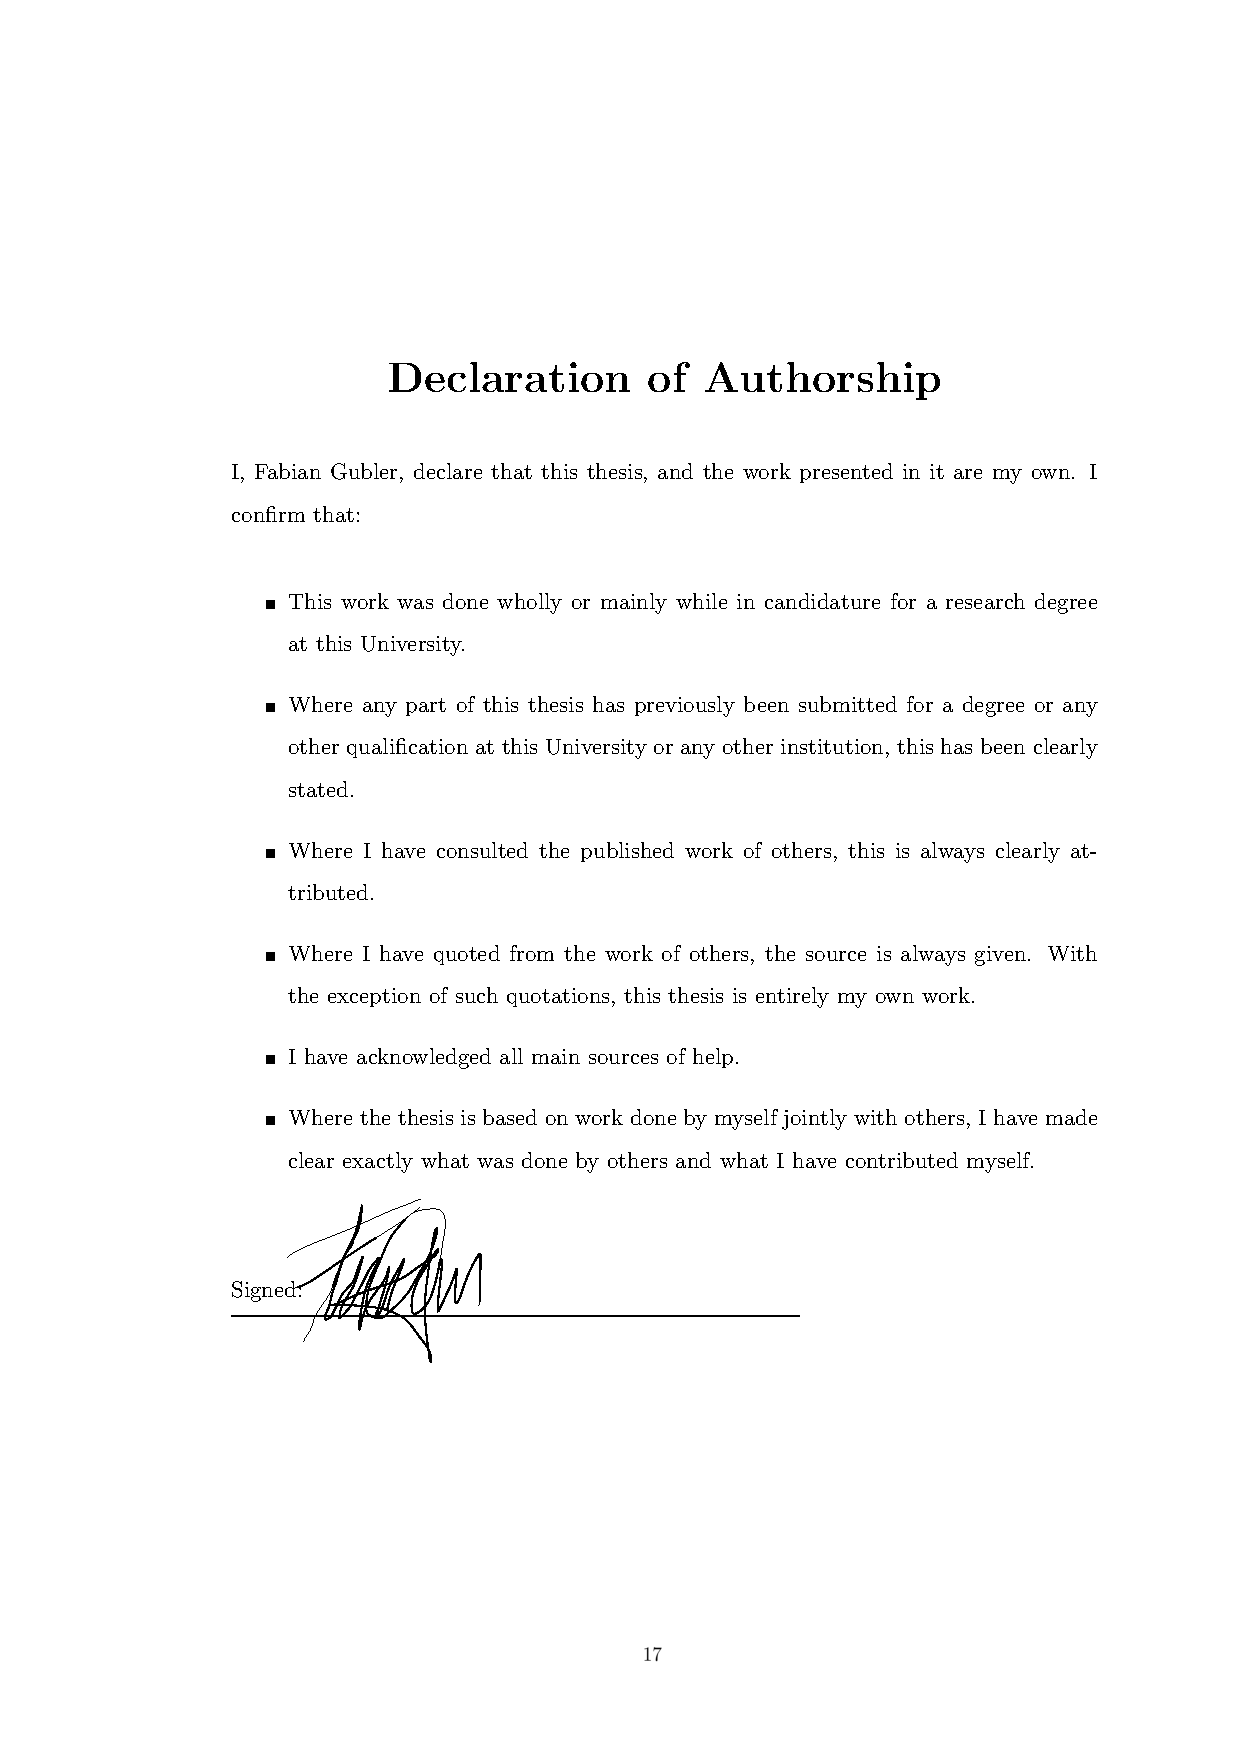
\includepdf[pages=-, offset=75 -75]{signed.pdf}

%% ----------------------------------------------------------------
% Now begin the Appendices, including them as separate files

\addtocontents{toc}{\vspace{2em}} % Add a gap in the Contents, for aesthetics

\appendix % Cue to tell LaTeX that the following 'chapters' are Appendices

\chapter{Appendix A}
\lhead{\emph{Appendix A}}  % Set the left side page header

Lorem Ipsum
	% Appendix Title
\chapter{Appendix B}
\lhead{\emph{Appendix B}}  % Set the left side page header
 % Appendix Title

\addtocontents{toc}{\vspace{2em}}  % Add a gap in the Contents, for aesthetics
\backmatter

%% ----------------------------------------------------------------
\label{Bibliography}
\lhead{\emph{Bibliography}}  % Change the left side page header to "Bibliography"
\bibliographystyle{unsrtnat}  % Use the "unsrtnat" BibTeX style for formatting the Bibliography
\bibliography{Bibliography}  % The references (bibliography) information are stored in the file named "Bibliography.bib"

\end{document}  % The End
%% ----------------------------------------------------------------
